\documentclass[a4paper,12pt]{article}
\usepackage[utf8]{inputenc}
\usepackage[slovene]{babel}
\usepackage{amsmath}
\usepackage{amsfonts}
\usepackage{amssymb}
\usepackage{graphicx}
\usepackage{geometry}

\title{Apex Garaza}
\author{Tjaž Pahor, Jakob Šimunić}
\date{November 2026}
\begin{document}

\maketitle
\tableofcontents

\section{Uvod}
Projekt \textbf{Apex Garaža} je zasnovan kot spletna platforma izmišljene avtohiše, specializirane za prodajo rabljenih športnih avtomobilov. Glavni problem, ki ga z rešitvijo naslavljava, je pomanjkanje preglednih in zanesljivih podatkov o dejanskem stanju vozila ter opravljenih servisih na obstoječih oglasnikih. Kupci športnih vozil se pri nakupu pogosto soočajo s pomanjkljivimi opisi in skrito zgodovino vzdrževanja. Namen najine platforme je kupcem omogočiti jasen vpogled v servisno zgodovino, tehnične podatke, kakovostne fotografije ter enostaven dogovor za ogled ali testno vožnjo prek spletnega kontaktnega obrazca.

%================================================================================
\section{Pregled obstoječih rešitev}

\subsection{Avto.net}
\textbf{Kratek opis:} Avto.net je največji slovenski spletni oglasnik za nakup in prodajo osebnih, gospodarskih in športnih vozil \cite{avtonet}. 

\textbf{Ključne funkcionalnosti:}
\begin{itemize}
    \item Napredno filtriranje oglasov po znamki, modelu, letniku, ceni, prevoženih kilometrih in moči motorja.
    \item Objava oglasov s fotografijami, osnovnimi tehničnimi podatki in prostim opisom prodajalca.
    \item Prikaz kontaktnih podatkov prodajalca ter možnost pošiljanja povpraševanja prek spletnega obrazca.
\end{itemize}

\textbf{Prednosti:}
\begin{itemize}
    \item Zelo velika izbira vozil na slovenskem trgu in visoka prepoznavnost.
    \item Hitro in preprosto iskanje po osnovnih tehničnih parametrih.
\end{itemize}

\textbf{Slabosti:}
\begin{itemize}
    \item Podatki o servisni zgodovini niso strukturirani in so odvisni izključno od dobre volje prodajalca v prostem besedilu.
    \item Zastarel uporabniški vmesnik in veliko število oglasov slabše kakovosti brez preverjenih podatkov o stanju vozila.
\end{itemize}

\begin{figure}[h]
    \centering
    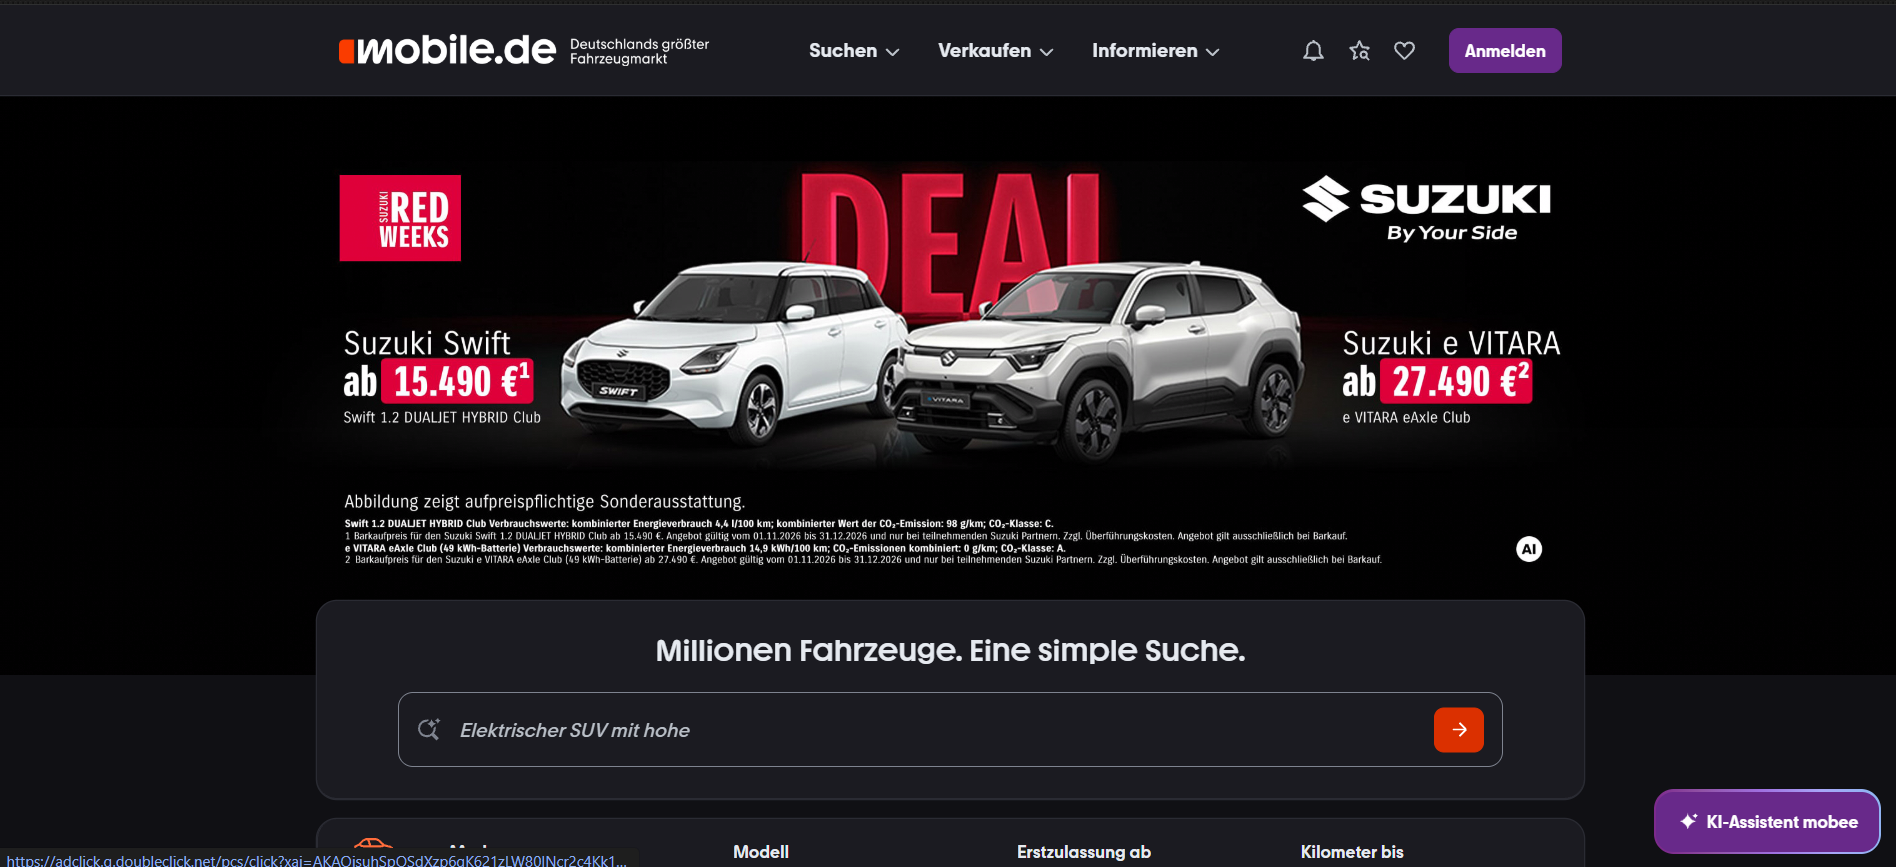
\includegraphics[width=0.85\textwidth]{avto.net.png}
    \caption{Avto.net \cite{avtonet}.}
    \label{fig:avtonet}
\end{figure}

%======================================================================================
\subsection{Mobile.de}
\textbf{Kratek opis:} Mobile.de je eden največjih evropskih spletnih portalov za trgovanje z rabljenimi in novimi vozili, ki ponuja tudi zelo bogat nabor zmogljivih in redkejših športnih avtomobilov \cite{mobilede}.

\textbf{Ključne funkcionalnosti:}
\begin{itemize}
    \item Podrobni filtri za opremo, vrsto pogona, menjalnik, zgodovino lastništva in oceno cene glede na trg.
    \item Prikaz ocen prodajalcev s strani preteklih kupcev.
    \item Shranjevanje priljubljenih oglasov in primerjava izbranih vozil.
\end{itemize}

\textbf{Prednosti:}
\begin{itemize}
    \item Ogromna ponudba športnih vozil z natančnimi filtri za opremo in tehnične lastnosti.
    \item Realna ocena cene
\end{itemize}

\textbf{Slabosti:}
\begin{itemize}
    \item Zaradi velikega števila filtrov in informacij je vmesnik za povprečnega uporabnika lahko nepregleden.
    \item Kljub obsežnim opisom ni enotnega standarda za preverjen prikaz celotne servisne zgodovine pri vsakem vozilu.
\end{itemize}

\begin{figure}[h]
    \centering
    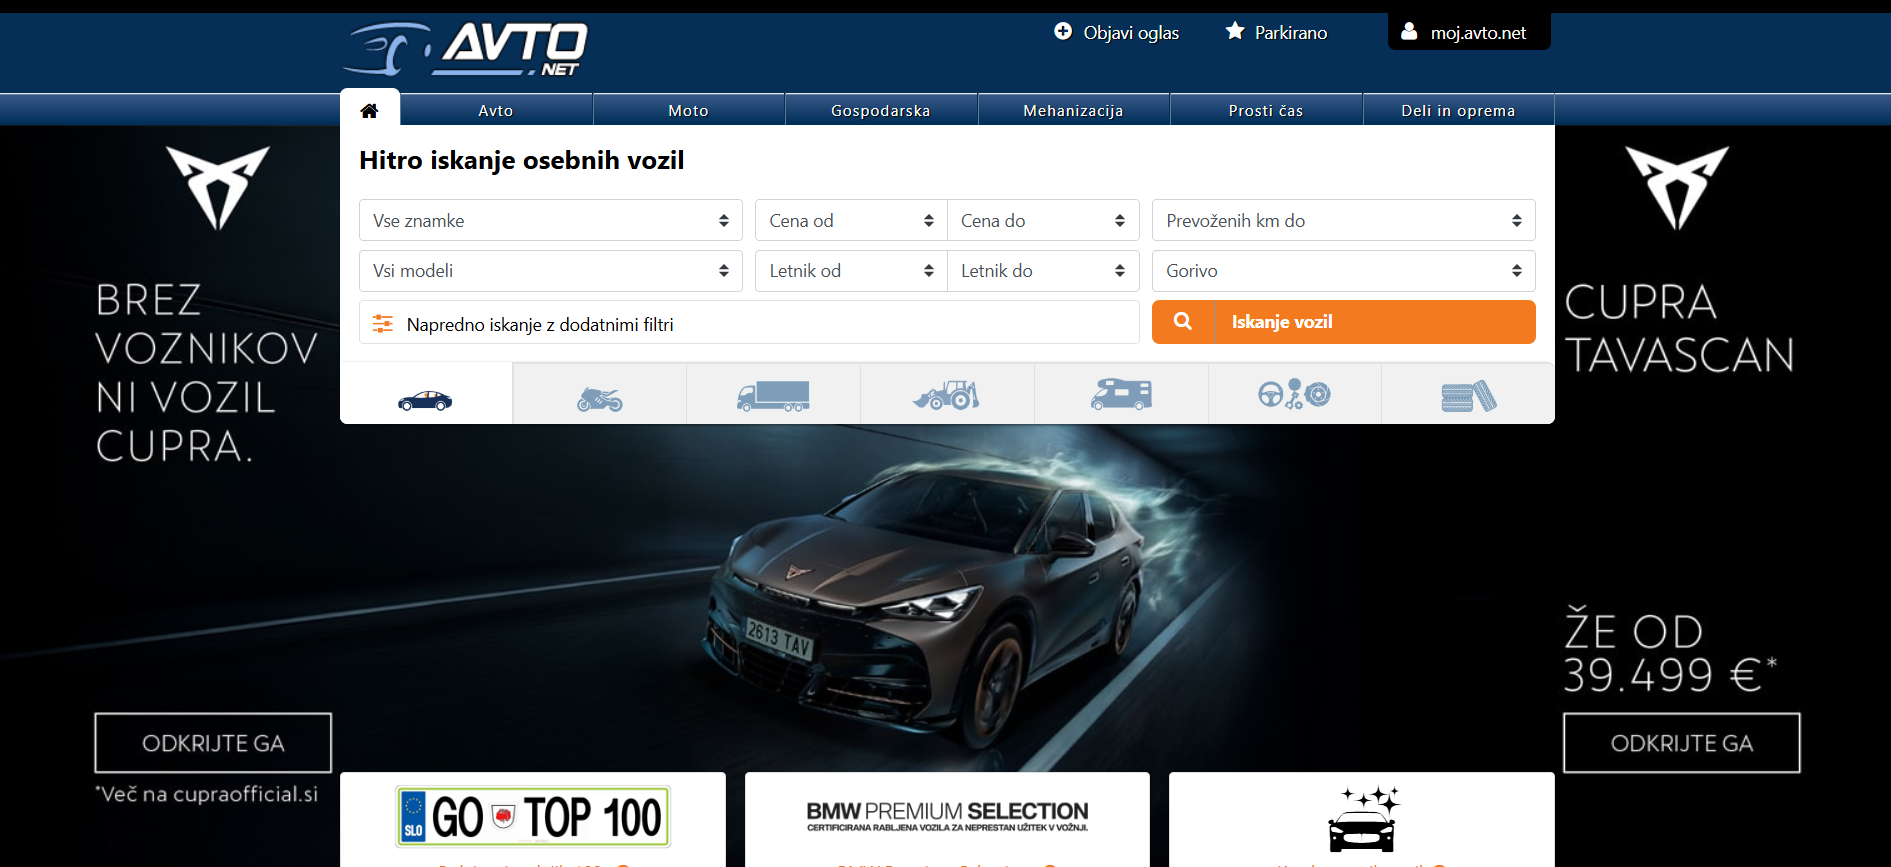
\includegraphics[width=0.85\textwidth]{mobile.de.png}
    \caption{Mobile.de \cite{mobilede}.}
    \label{fig:mobilede}
\end{figure}

%==================================================================================
\subsection{Carfax}
\textbf{Kratek opis:} Carfax je specializirana spletna storitev za preverjanje zgodovine rabljenih vozil na podlagi identifikacijske številke vozila \cite{carfax}. Namenjena je zmanjševanju tveganja pri nakupu rabljenega avtomobila.

\textbf{Ključne funkcionalnosti:}
\begin{itemize}
    \item Generiranje poročila o zgodovini vozila na podlagi številke šasije.
    \item Prikaz zapisov o preteklih poškodbah, številu lastnikov in zabeleženih prevoženih kilometrih.
    \item Vpogled v zabeležene servisne posege in tehnične preglede.
\end{itemize}

\textbf{Prednosti:}
\begin{itemize}
    \item Visoka stopnja zaupanja zaradi uradnih in preverjenih zapisov o stanju vozila.
    \item Jasno in strukturirano poročilo, ki kupcu pomaga prepoznati morebitne skrite napake ali prevrtene kilometre.
\end{itemize}

\textbf{Slabosti:}
\begin{itemize}
    \item Storitev je plačljiva za vsako posamezno poizvedbo in ni brezplačno vključena v sam oglas.
    \item Ne omogoča neposrednega nakupa vozila ali dogovora za testno vožnjo, saj služi le kot zunanje orodje za preverjanje.
\end{itemize}

\begin{figure}[h]
    \centering
    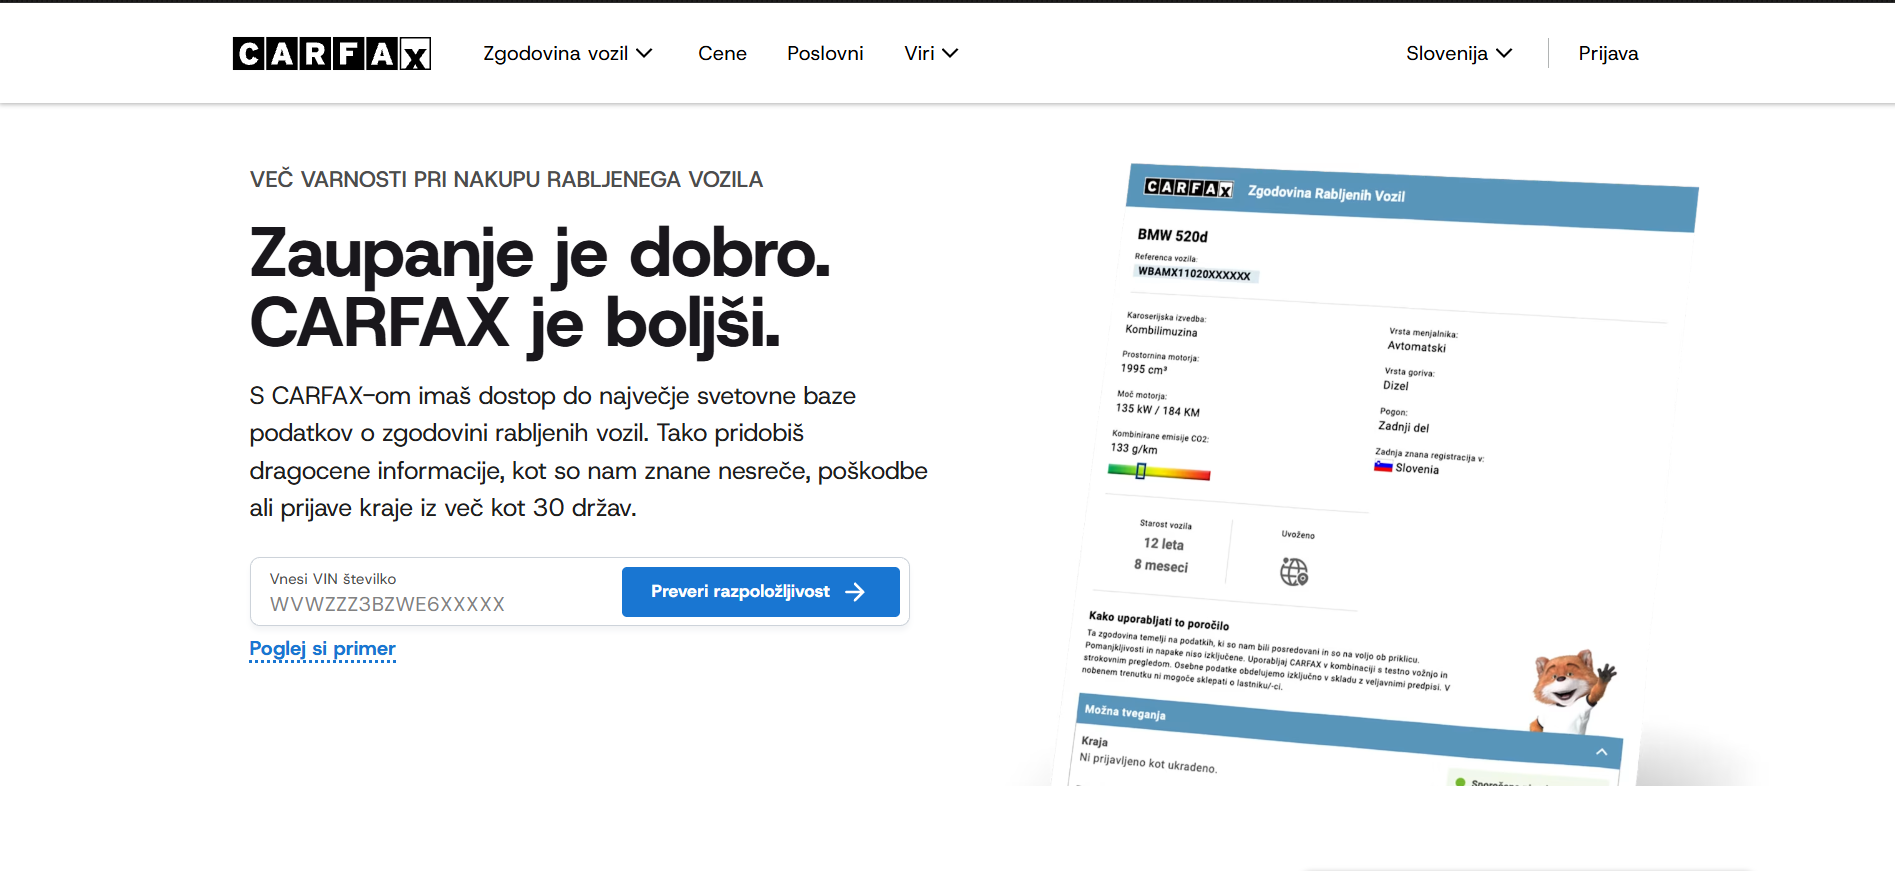
\includegraphics[width=0.85\textwidth]{carfax.png}
    \caption{Carfax \cite{carfax}.}
    \label{fig:carfax}
\end{figure}


%===================================================================================
\section{Zaključek}
Iz analiziranih rešitev bova za platformo Apex Garaža prevzela najboljše prakse vsake izmed njih. Od portalov Avto.net in Mobile.de bova prevzela pregleden katalog s ključnimi tehničnimi filtri ter možnost neposrednega kontaktiranja prodajalca. Od storitve Carfax pa bova prevzela idejo strukturiranega in preglednega prikaza servisne zgodovine ter stanja vozila. Najina rešitev bo to naredila bolje in drugače predvsem v tem, da bodo preverjeni podatki o opravljenih servisih in tehničnem stanju vozila že pred ogledom, brez potrebe po plačevanju zunanjih poročil. Poleg tega bo platforma specializirana izključno za športne avtomobile, z modernim, čistim uporabniškim vmesnikom, enostavno primerjavo modelov in hitrim obrazcem za rezervacijo testne vožnje.


\begin{thebibliography}{9}

\bibitem{avtonet}
Avto.net. \emph{Največji slovenski avtomobilski oglasnik}. Dostopno na: \url{https://www.avto.net/} (pridobljeno: november 2026).

\bibitem{mobilede}
Mobile.de. \emph{Deutschlands größter Fahrzeugmarkt}. Dostopno na: \url{https://www.mobile.de/} (pridobljeno: november 2026).

\bibitem{carfax}
Carfax Europe. \emph{Preverite zgodovino rabljenega vozila}. Dostopno na: \url{https://www.carfax.eu/} (pridobljeno: november 2026).

\end{thebibliography}



\end{document}
